\documentclass[../design_fonctionnement_sys.tex]{subfiles}
\begin{document}

\section{Design du système}
Le système est divisé en 7 entités:
\begin{itemize}
    \item Client (en gris)
    \item Connexion et Inscription (en rose)
    \item Menu principal (en jaune)
    \item ModeCommande (en bleu ciel)
    \item Lobby (en orange)
    \item Chat (en vert)
    \item Jeu (en bleu foncé)
    \item Database (en rouge)
    \newline
\end{itemize}

Nous allons les détailler dans différents diagrammes. A noter que toutes ces entités vont hériter des mêmes classes abstraites.
Cela est du au fait d'utiliser le design MVC pour cette application.
Chaque entité du système est donc composée de 3 composantes principales:
\begin{itemize}
    \item La vue: Elle correspond à l'interface, elle permet d'afficher les informations 
    et de reçevoir les input de l'utilisateur qu'elle communique au controller.
    \item Le controller: Il gère les requètes envoyées par la vue et les communique au serveur avec lequel il échange des informations.
    Il met le serveur à jour suite aux actions d'utilisateurs.
    \item Le serveur: il contient toutes les informations relatives aux utilisateur et à une partie. 
    Il est responsable d'envoyer les informations requise par le controller et permet de mettre les joueurs en relation pour une partie.\\
\end{itemize}

En partie, chaque client est connecté au même plateau, et à son propre côté. Le game serveur fait le lien entre les deux.
Le gameController permet de mettre à jour le plateau de chaque client après une action.

\newpage
\subsection{Client}
Les classes abstraites Vue, Console et GUI jouent un rôle essentiel dans l'affichage des divers écrans de l'application, 
offrant ainsi une expérience utilisateur flexible soit en ligne de commande, soit à travers une interface graphique. 
La classe abstraite Controller sert à valider les saisies des utilisateurs avant de les transmettre au serveur, 
garantissant ainsi la cohérence et la sécurité des données échangées. 
Par ailleurs, la classe GameClient permet à l'application de se connecter au serveur et de lui soumettre des requêtes, 
assurant ainsi la communication fluide entre l'utilisateur et le système distant. 
Enfin, la classe Driver agit comme un pont entre toutes ces classes, orchestrant leur interaction harmonieuse pour offrir une expérience utilisateur complète et cohérente.
\begin{figure}[H]
    \centering
    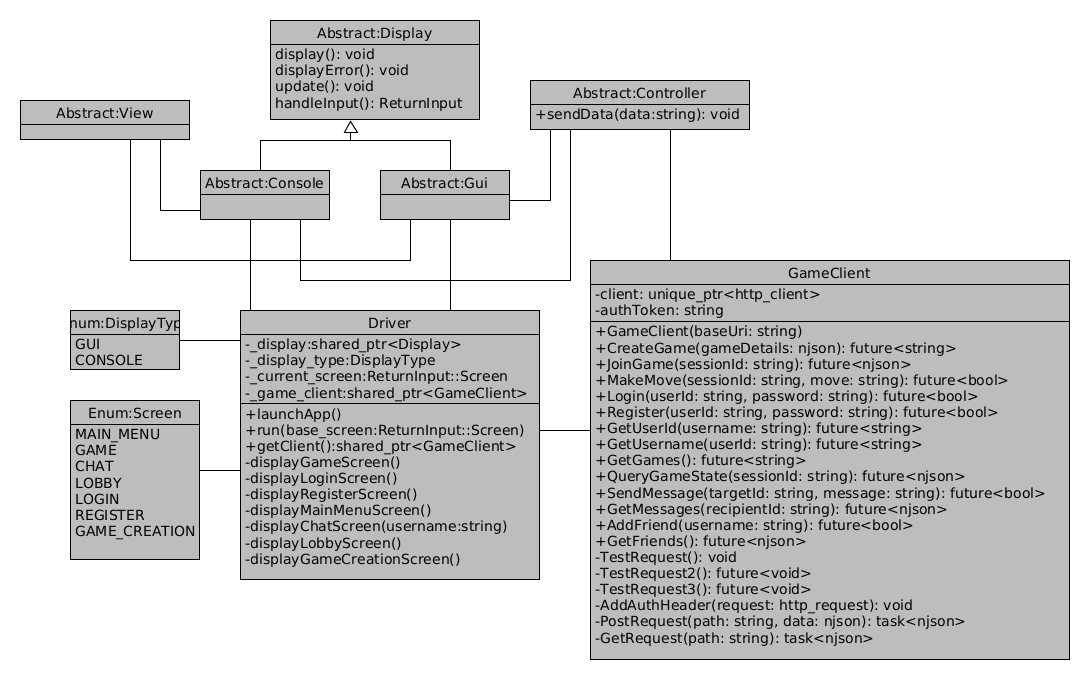
\includegraphics[scale=0.4]{img_design/client_design.png}
    \label{fig:client}
    \caption{Client}
\end{figure}

\newpage
\subsection{Connexion et Inscription}
Dès que le joueur lance le jeu, il a la possibilité de soit créer un compte, soit se connecter au compte qu'il a déjà. 
Il aura donc deux interfaces différentes pour ces deux actions.
\begin{figure}[H]
    \centering
    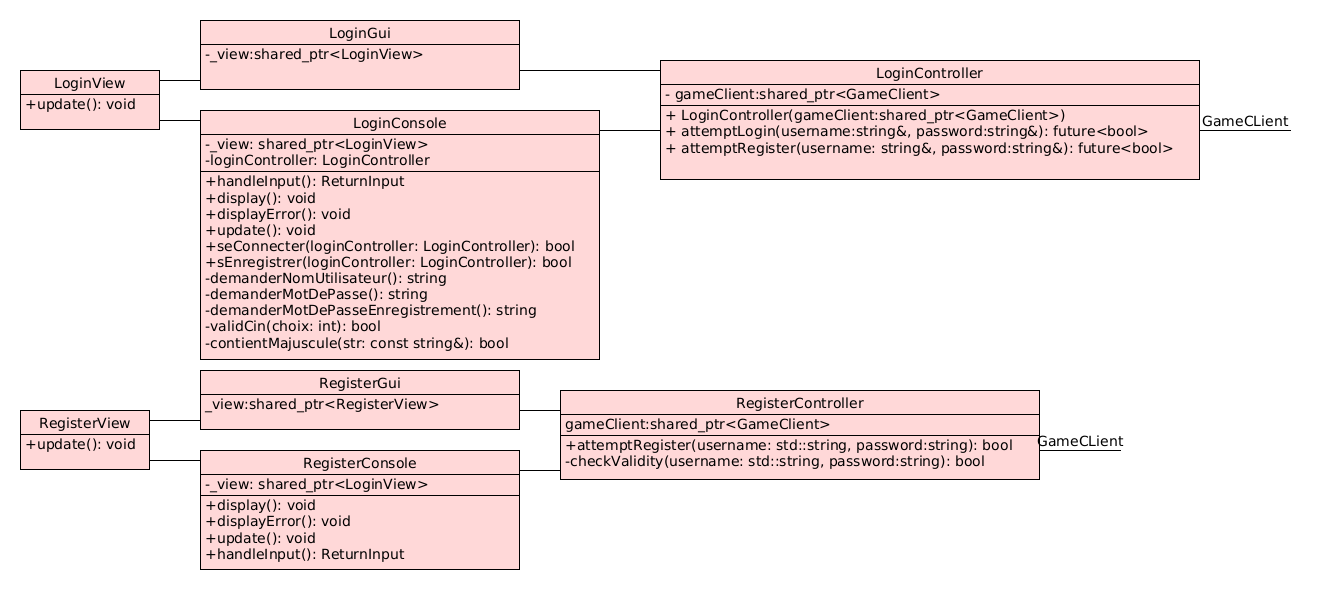
\includegraphics[scale=0.3]{img_design/4.2_login_register_design.png}
    \label{fig:seq_match_server}
    \caption{Connexion et Inscription}
\end{figure}

\subsection{Menu principal}
Le menu principal est celui qui permettra d'accéder aux autres écrans du jeu, tels que la création de partie, ou la modification de profil.
\begin{figure}[H]
    \centering
    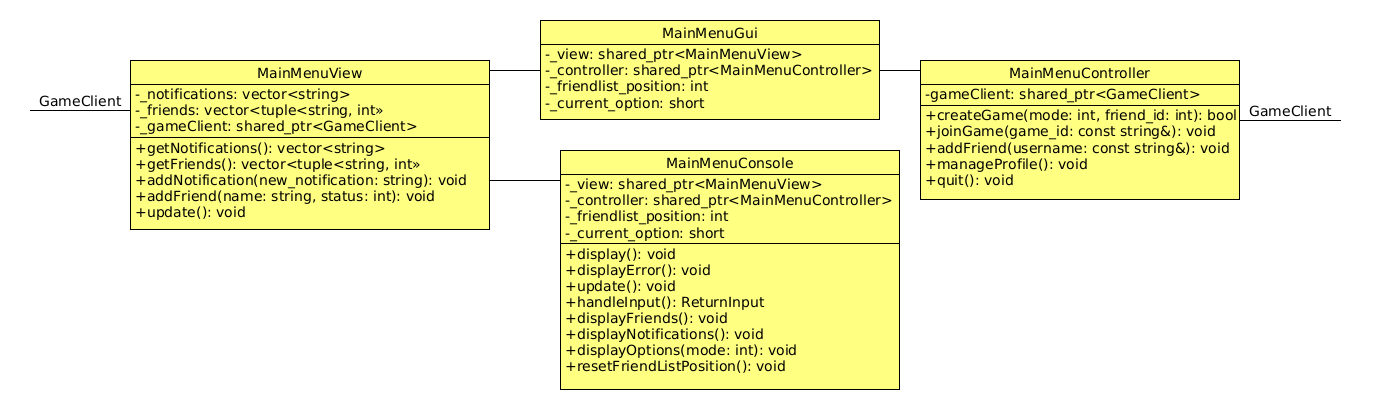
\includegraphics[scale=0.3]{img_design/4.4_mainmenu_design.png}
    \label{fig:seq_match_server}
    \caption{Menu principal}
\end{figure}

\newpage
\subsection{Mode Commandant}
Le mode Commandant est une option de jeu spéciale qui permet aux joueurs de choisir une faction de bateaux unique et d'accéder à des actions spéciales pour influencer les batailles navales. 

\begin{figure}[H]
    \centering
    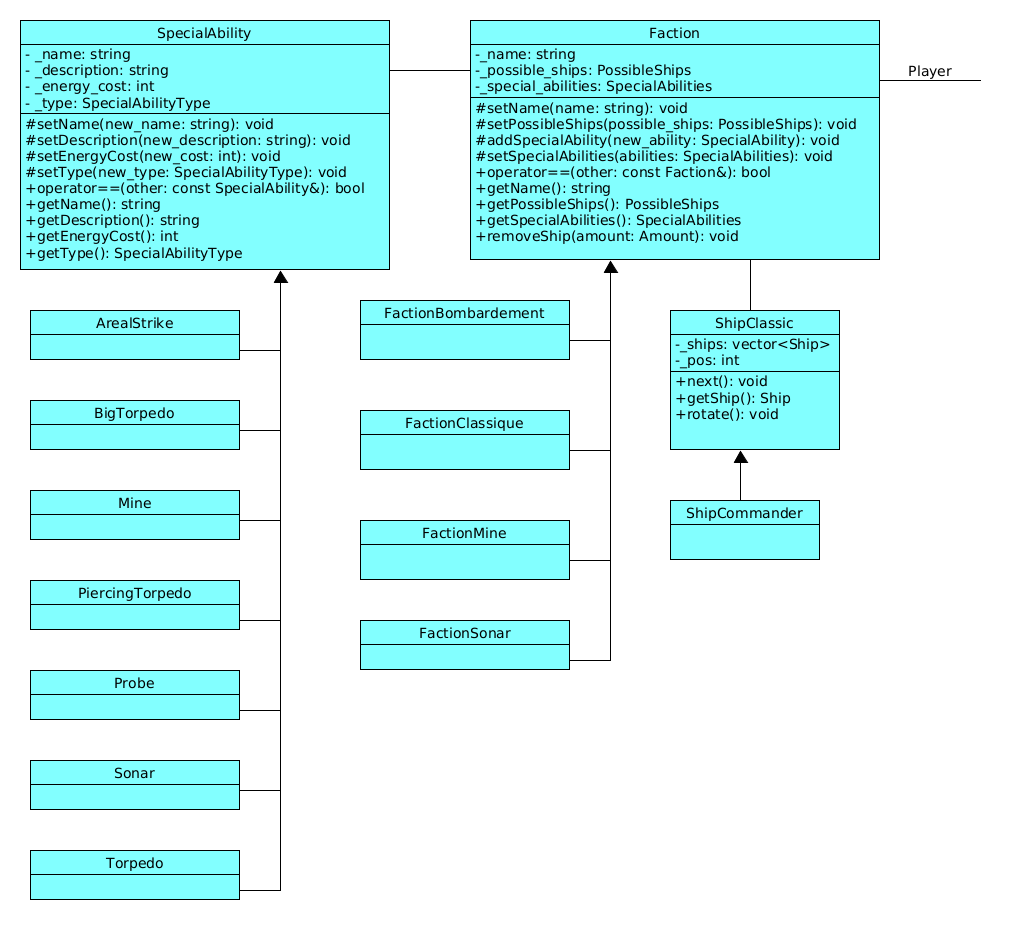
\includegraphics[scale=0.4]{img_design/mode_commandant.png}
    \label{fig:seq_match_server}
    \caption{Gestion des comptes}
\end{figure}

\newpage
\subsection{Loby}
En lançant une partie, un joueur rejoint le lobby en attendant que les autres joueurs et spectateurs se joignent à celle-ci. \begin{figure}[H]
    \centering
    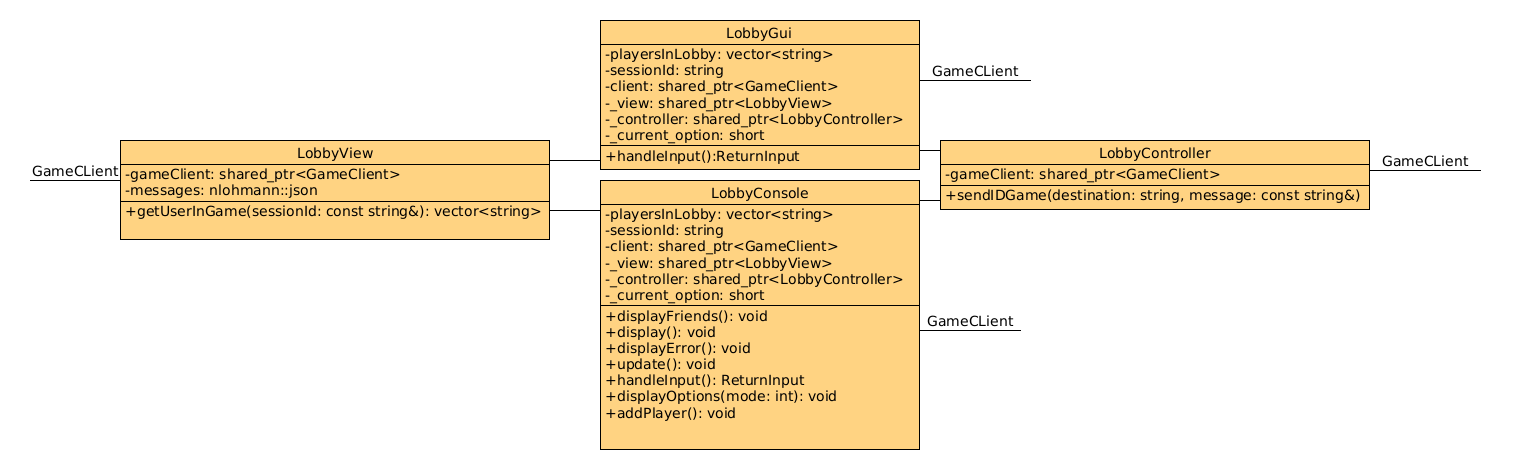
\includegraphics[scale=0.3]{img_design/4.6_lobby_design.png}
    \label{fig:seq_match_server}
    \caption{Profil}
\end{figure}

\subsection{Chat}
Le jeu offre aux joueurs un chat qui leur permet d'envoyer une chaine de caractère qui sera envoyée à tous les autres joueurs. 
\begin{figure}[H]
    \centering
    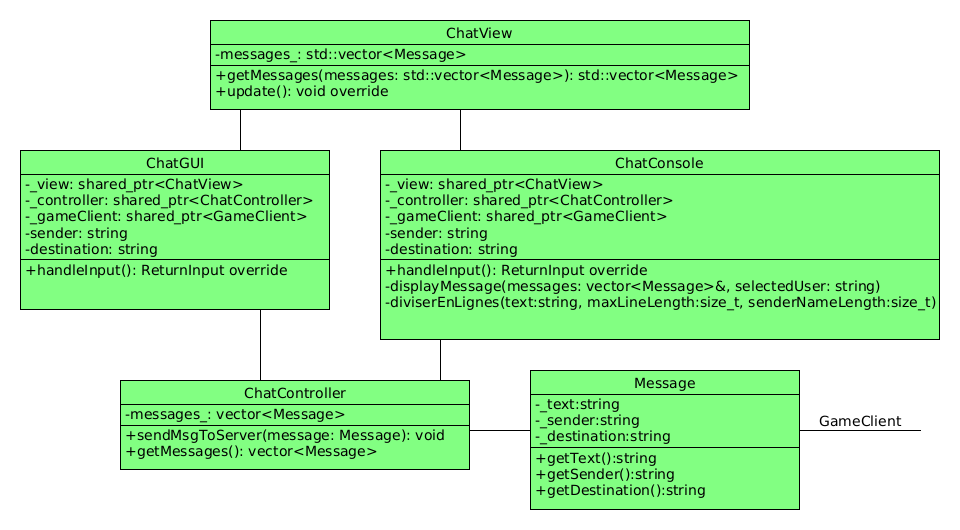
\includegraphics[scale=0.3]{img_design/4.7_chat_design.png}
    \label{fig:seq_match_server}
    \caption{Chat}
\end{figure}

\newpage
\subsection{Jeu}
\subsubsection{Affichage du jeu}
La partie locale du jeu est concue de la manière suivante: 
le joueur a une board local qui est une copie du board du serveur (avec les cases de l'adversaire qui sont masquées), 
un controlleur qui permet de communiquer avec le serveur et un display qui permet d'afficher une partie à l'écran.
\begin{figure}[H]
    \centering
    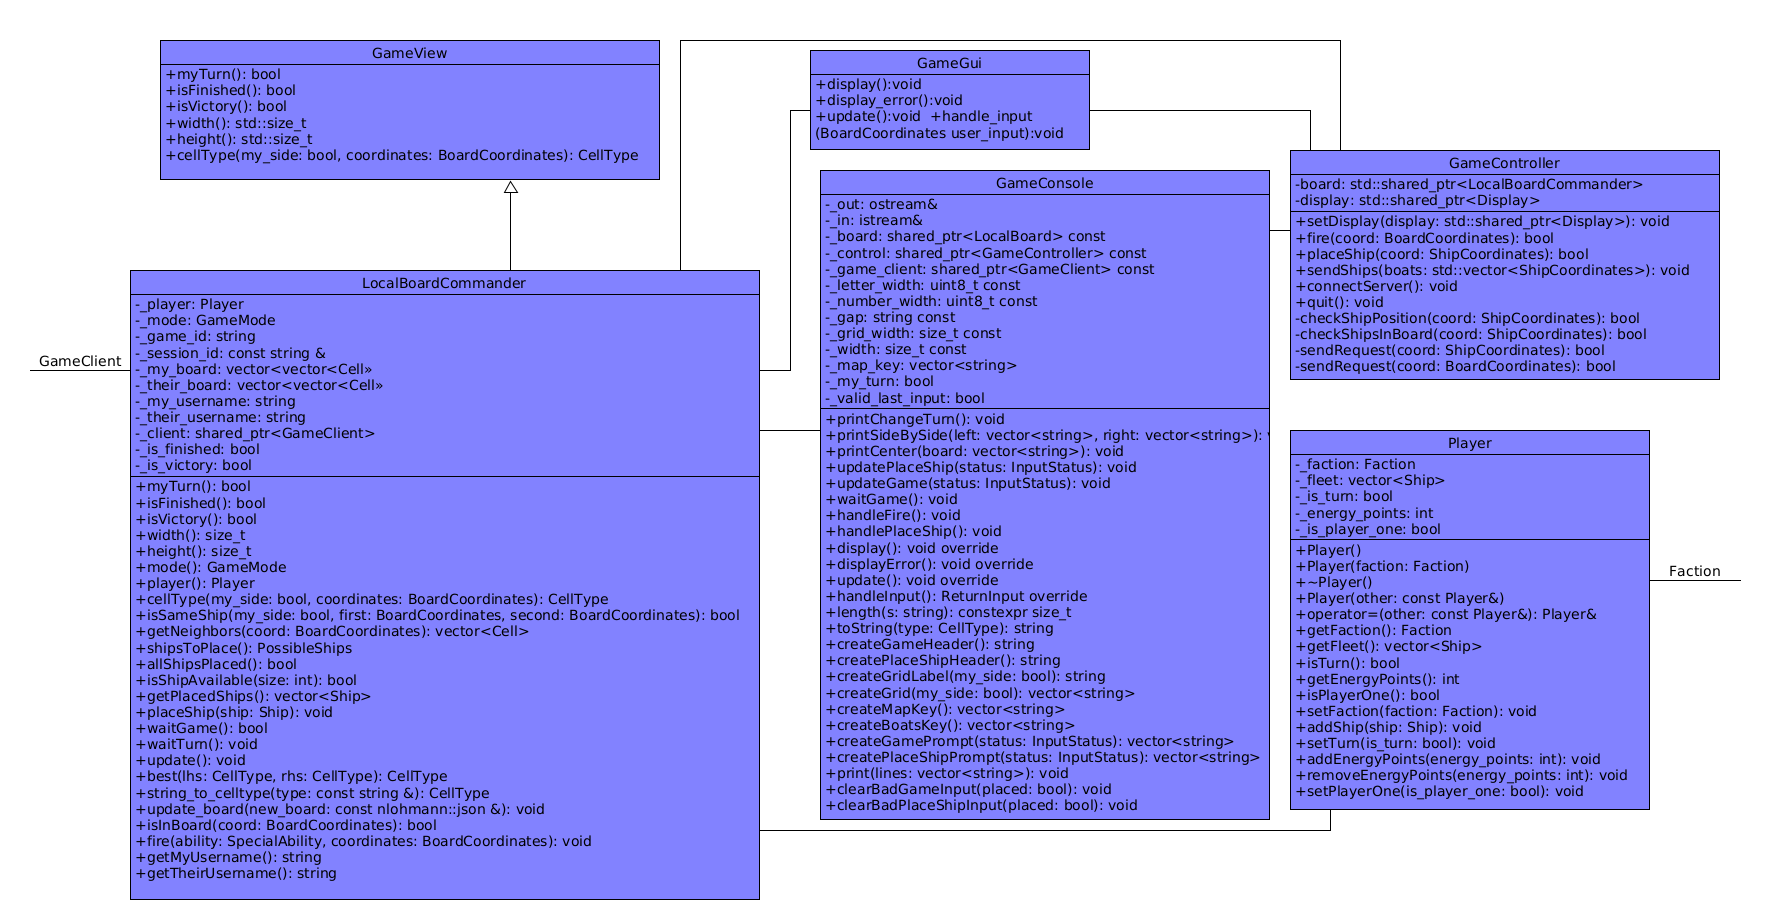
\includegraphics[scale=0.2]{img_design/4.8_affichage_game.png}
    \label{fig:seq_match_server}
    \caption{Game affichage}
\end{figure}

\newpage
\subsubsection{Game server}
La partie distante du jeu est gérée par une classe GameServer, chargée de réaliser les requêtes auprès de la base de données, 
de les communiquer au GameClient et de fournir des tokens d'identification. À chaque partie, le GameServer crée une session de jeu gérée par le SessionManager. 
La GameSession se charge de créer un état de jeu (gameState) ainsi qu'une instance de jeu (Game) contenant le plateau de jeu. Cette structure hiérarchique permet une gestion efficace et organisée des parties en ligne.
\begin{figure}[H]
    \centering
    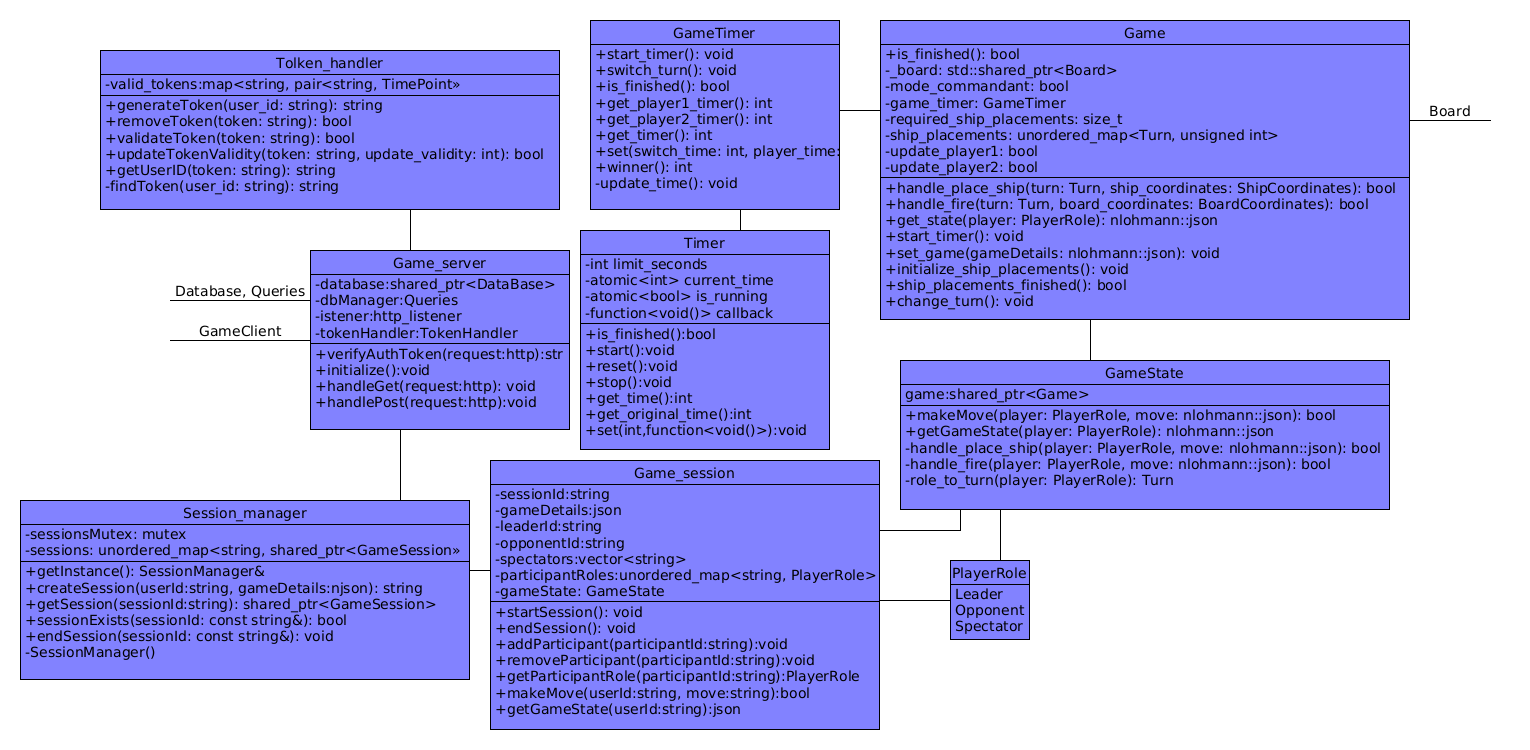
\includegraphics[scale=0.3]{img_design/4.9.1_game_server_design.png}
    \label{fig:seq_match_server}
    \caption{Game Server}
\end{figure}

\newpage
\subsubsection{Plateau de jeu}
En ce qui concerne la partie serveur d'une partie, nous avons une instance de Board qui contient les plateaux des deux joueurs, 
ainsi qu'une flotte qui appartient à ces deux joueurs. Le GameServeur est la classe qui s'occupe de la communication entre le Board et les joueurs.
\begin{figure}[H]
    \centering
    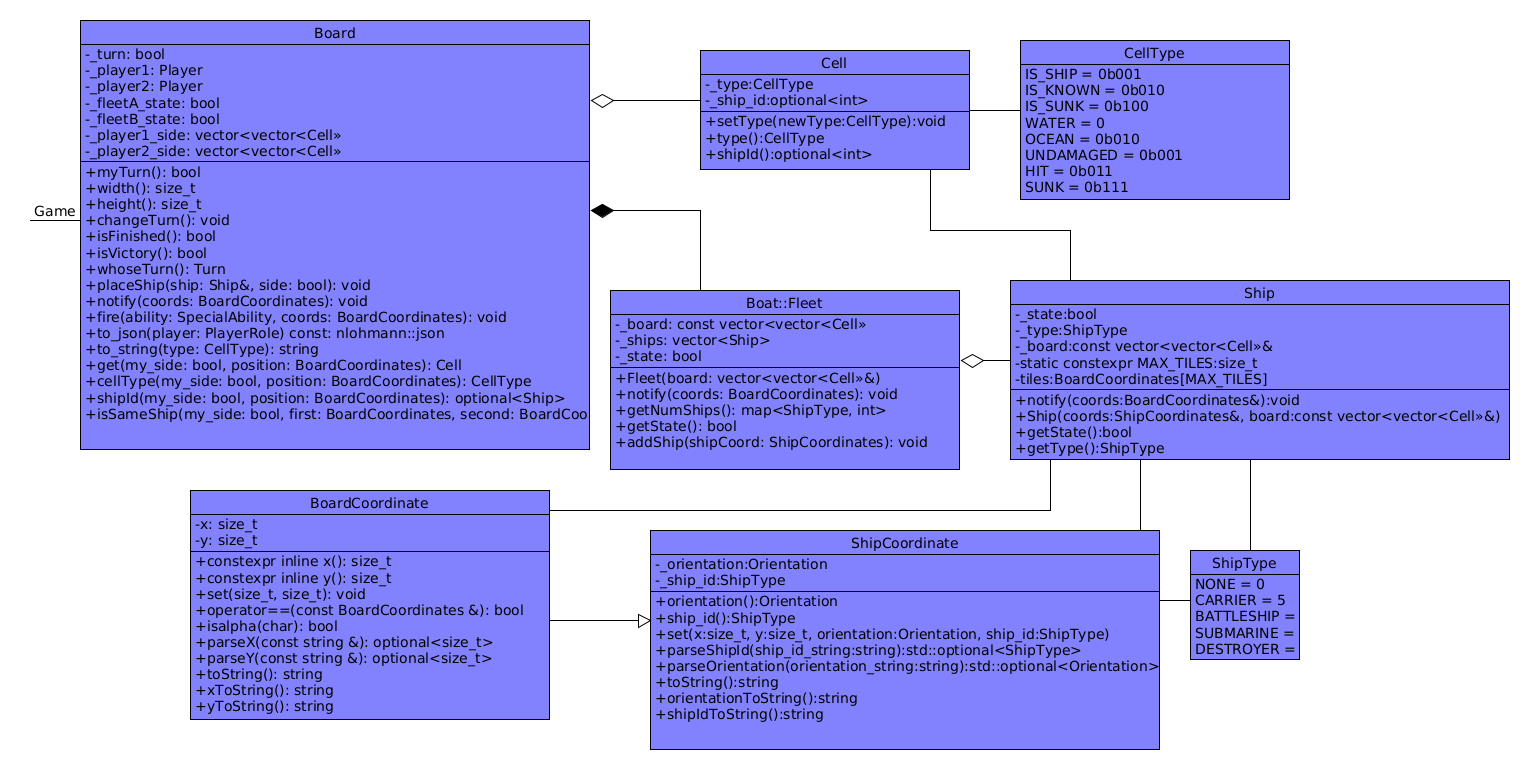
\includegraphics[scale=0.3]{img_design/4.9.2_board_design.png}
    \label{fig:seq_match_server}
    \caption{Game Board}
\end{figure}

\newpage
\subsection{Database}
La base de données stocke les informations utilisateur telles que le nom d'utilisateur, 
le mot de passe hashé, la liste d'amis et les messages.
La base de données est composée d'une classe Database effectuant les opérations de base telles que l'insertion et la sélection de données, 
ainsi que d'une classe Queries qui manipule la classe Database pour soumettre des requêtes spécifiques à l'application. 
Ces classes renvoient des instances de QueryResult, permettant de gérer les erreurs liées à la base de données et le résultat des requêtes de manière efficace.
\begin{figure}[H]
    \centering
    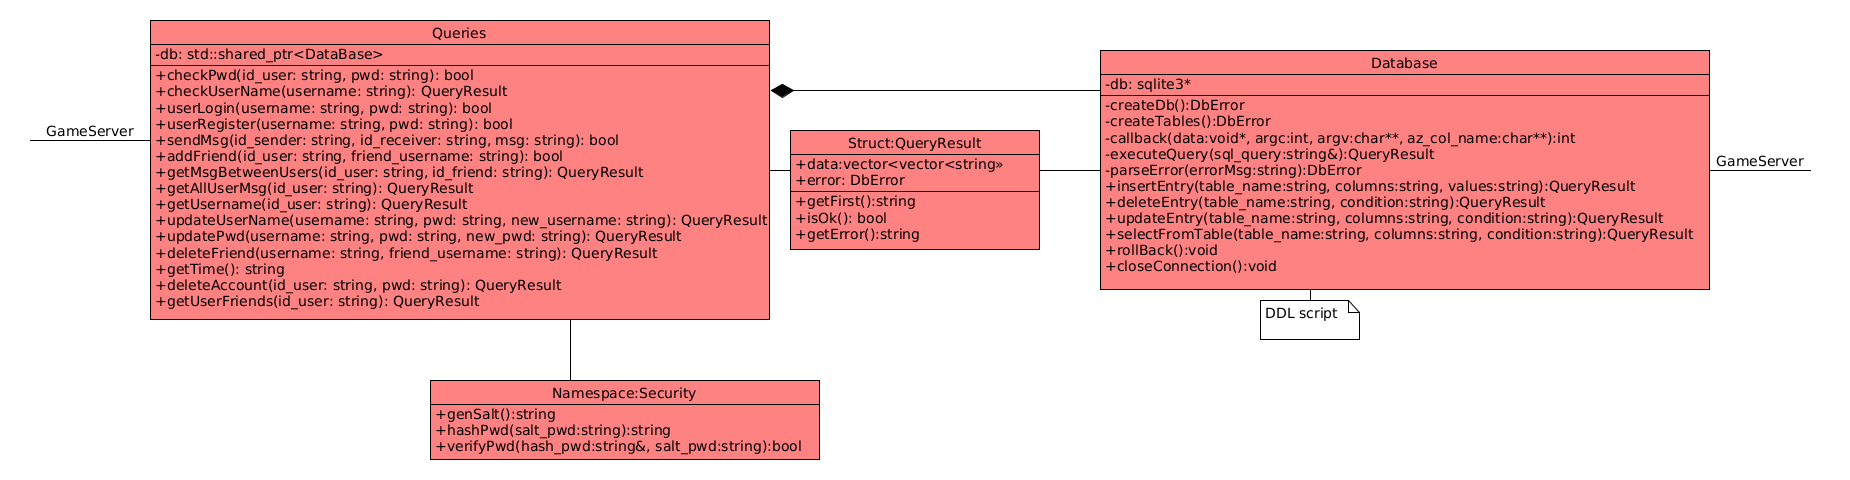
\includegraphics[scale=0.25]{img_design/dia_db.png}
    \label{fig:seq_match_server}
    \caption{Database}
\end{figure}

\end{document}
